\begin{task}{3, Using the console interface from Vadere}
This task aims to explore the utilization of the Vadere simulation software's console interface, allowing for the modification of scenario files and the addition of pedestrians through programming. Leveraging the console version enables Vadere's use as a "black box" within alternative software environments, such as Python.

The primary objective of this task is to programmatically add pedestrian to scenario files and compare the results between the console version and the graphical user interface. The "corner scenario" will be employed as the initial scenario, and the code will be developed to add pedestrians to specific locations. By comparing runtimes, we aim to discuss the similarities and differences in reaching the target between the added pedestrians and those originating from the source area.

\paragraph{add\_pedestrian.py}
To modify the Vadere simulation scenario file programmatically in order to add pedestrian, we created a Python script (\texttt{Exercises-MLCMS-Group-C/Exercise-2/add\_pedastrian/add\_pedestrian.py}). Here's a concise overview of the implementation details:

\begin{itemize}
    \item \textbf{Predefined pedestrian template}
    \begin{itemize}
        \item We formulated a JSON template, representing the attributes of the pedestrian intended for addition to the scenario.
    \end{itemize}

    \item \textbf{Adding Pedestrian function}
    \begin{itemize}
        \item The heart of the implementation lies in a function:
        \begin{itemize}
            \item It reads the existing scenario file.
            \item Picked a unique ID for the newly introduced pedestrian.
            \item Updates the predefined pedestrian template with the ID and user-provided inputs.
            \item Appends the modified pedestrian template to the 'dynamicElements' list within the scenario file.
        \end{itemize}
    \end{itemize}
    
    \item \textbf{Setting Pedestrian Parameters}
    \begin{itemize}
        \item During script execution through the Command Line, users specify parameters such as the scenario path to be modified, the initial position of the pedestrian to be added, their speed, and the target ID.
    \end{itemize}
\end{itemize}

\paragraph{Workflow} 
    The following is the workflow for the task. For the sake of convenience, these commands has been  recorded in \texttt{Exercises-MLCMS-Group-C/Exercise-2/add\_pedastrian/task3.ipynb}
\\

\textbf{1. add pedestrian to RiMEA scenario 6}

    \begin{verbatim}
    python add_pedestrian.py 
    --scenario "..\\vadere-project-task\\scenarios\\RiMEA scenario 6.scenario" 
    --x 22 --y 3 --targetID 3 --speed 0.5
    \end{verbatim}

\textbf{2. call vadere-console.jar with the newly modified scenario file.}
    \begin{verbatim}
    $java -jar vadere-console.jar scenario-run
    --scenario-file "..\\vadere-project-task\\scenarios\\RiMEA scenario 6_modified.scenario" 
    --output-dir "..\\scenarios\\output"
    \end{verbatim}

\paragraph{Command vs GUI} 
    After executing the command, as compared to the GUI, the Command prints out log records detailing the initialization of the simulation scenario, analysis of the JSON tree, utilization of the configuration file, solving of the floor field, initialization of pedestrians, and the various stages of the simulation run. Additionally, the logs cover the generation of output files, including trajectory data, overlap information, and other relevant details.

    After completing the simulation run, four output files were generated in both GUI and Command Line executions. These files include:
    \begin{itemize}
        \item \texttt{overlapCount.txt}
        \item \texttt{overlaps.csv}
        \item \texttt{postvis.traj}
        \item \texttt{RiMEA scenario 6\_modified.scenario}
    \end{itemize}
    A thorough comparison of the content within these files reveals that the files generated through both interfaces are found to be identical in every aspect. It signifies the reliability and coherence of the Vadere. This consistency is valuable for users who may opt for either interface based on their preferences or specific workflow requirements, assuring them that the simulation results will remain consistent irrespective of the chosen mode of execution.

\paragraph{Comparing Pedestrian Travel Times}
In the graphical user interface scenario, Figure \ref{fastest1} illustrates that the pedestrian we added is the fastest to reach the destination.

Upon utilizing the \texttt{Command} to add a pedestrian, the system outputs: "Finished adding pedestrian. ID of the new pedestrian is 7." Consequently, we can use ID 7 to precisely locate the trajectory information of this newly added pedestrian in the \texttt{./vadere-project-task123/output/RiMEA scenario 6\_modified/postvis.traj} file. To isolate the trajectory details for the newly added pedestrian, we apply the regular expression \texttt{\textasciicircum(?!7).*\textbackslash n}, replacing all matching entries with empty strings. After restoring the first line of the original text, the resulting content, as shown in the figure \ref{fastest2}, encapsulates the entire trajectory information for the new pedestrian. Notably, this pedestrian completes its journey in 11 simulation unit time.

In contrast, pedestrians generated in the source area exhibit a broader range of travel times. The slowest pedestrian from the source area takes 69.55 simulation unit time to reach the destination, as indicated by the last line of the \texttt{postvis.traj} file \ref{slowest}. The fastest pedestrian from the source area completes the journey in 25.28 simulation unit time \ref{source_fast}. To extract this information, we employ regular expression repeatedly to remove entries containing IDs, those appearing in the last line. Ultimately, the remaining two entries consist of the newly added pedestrian and the one who from source area reached the fastest.

\begin{figure}[H] 
\centering
\subfigure[The Added pedestrian reaches exit in GUI\label{fastest1}]{
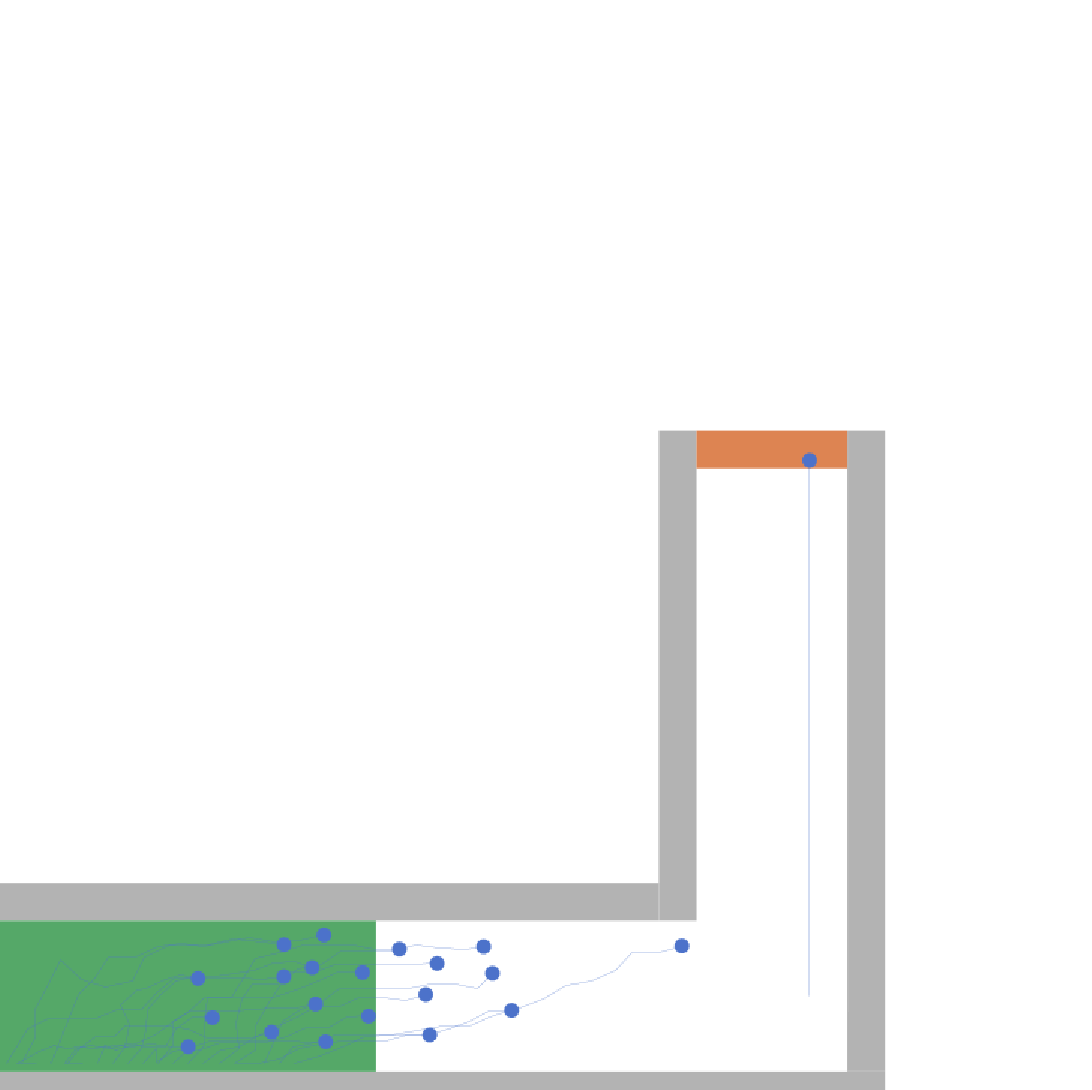
\includegraphics[scale=0.35]{report-template/images/fastest1.png}}
\subfigure[The Added pedestrian, ID 7\label{fastest2}]{
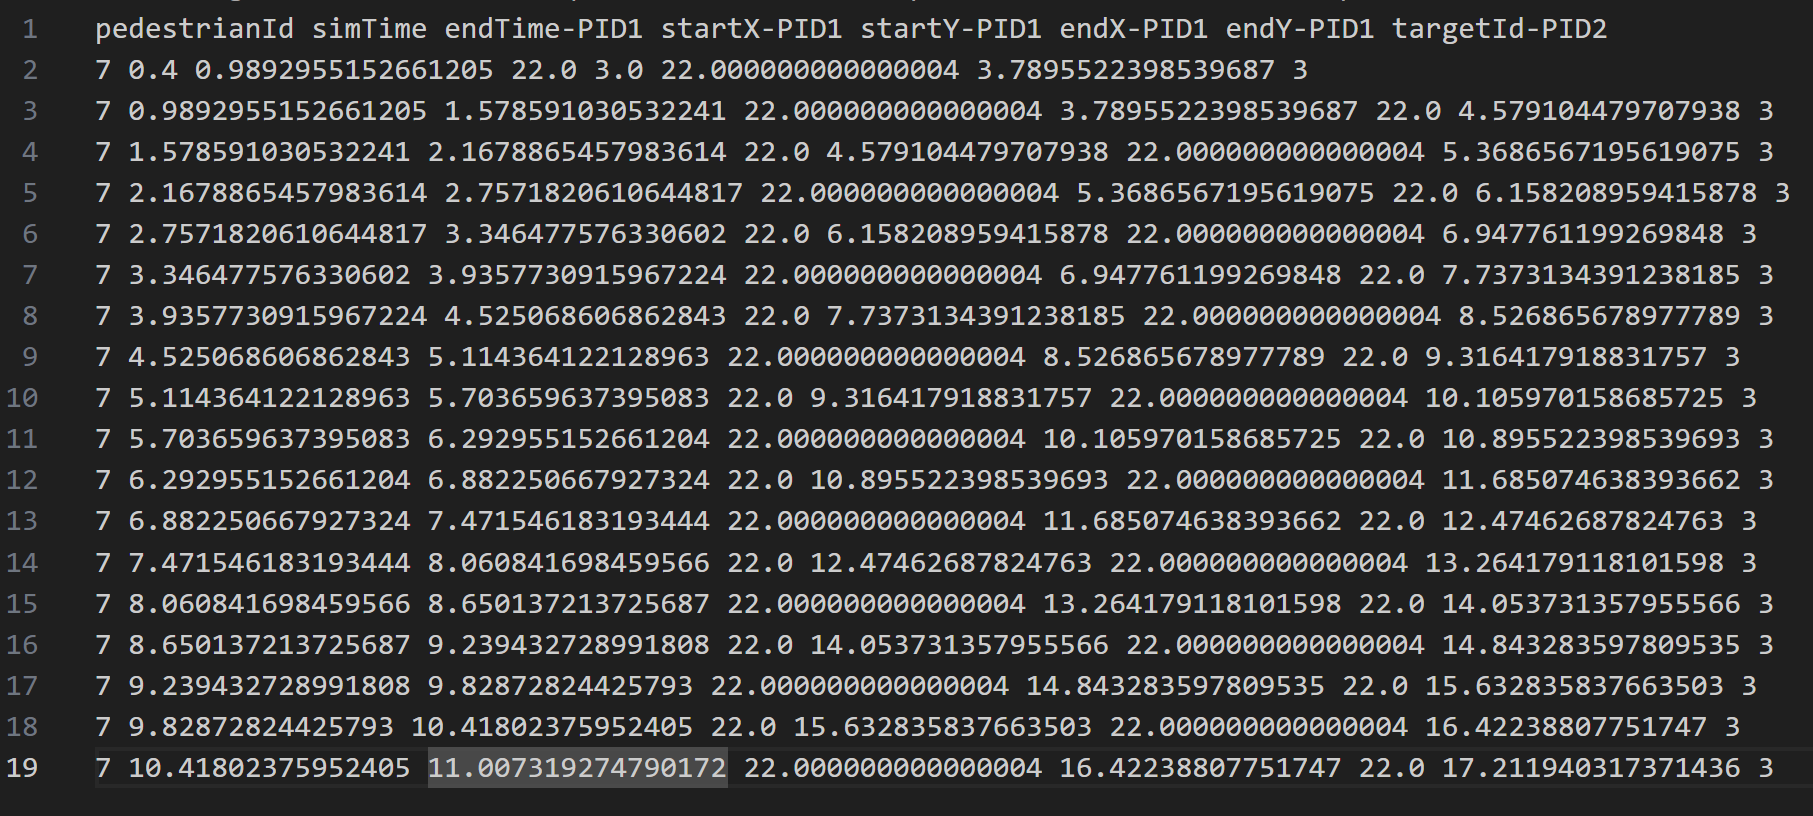
\includegraphics[scale=0.25]{report-template/images/fastest2.png}}
\subfigure[The slowest source pedestrian, ID 13\label{slowest}]{
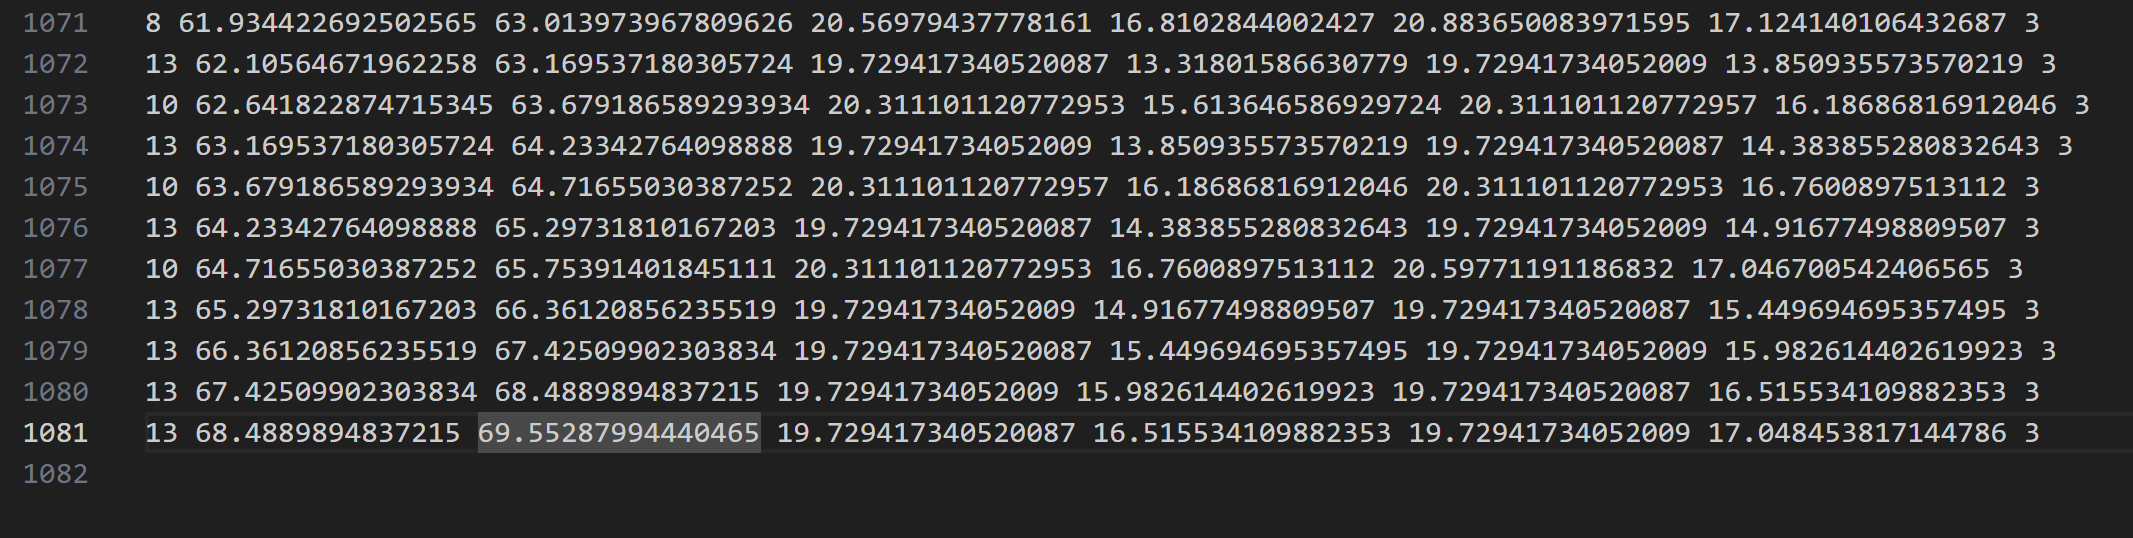
\includegraphics[scale=0.2]{report-template/images/slowest.png}}
\subfigure[The fastest source pedestrian, ID 27\label{source_fast}]{
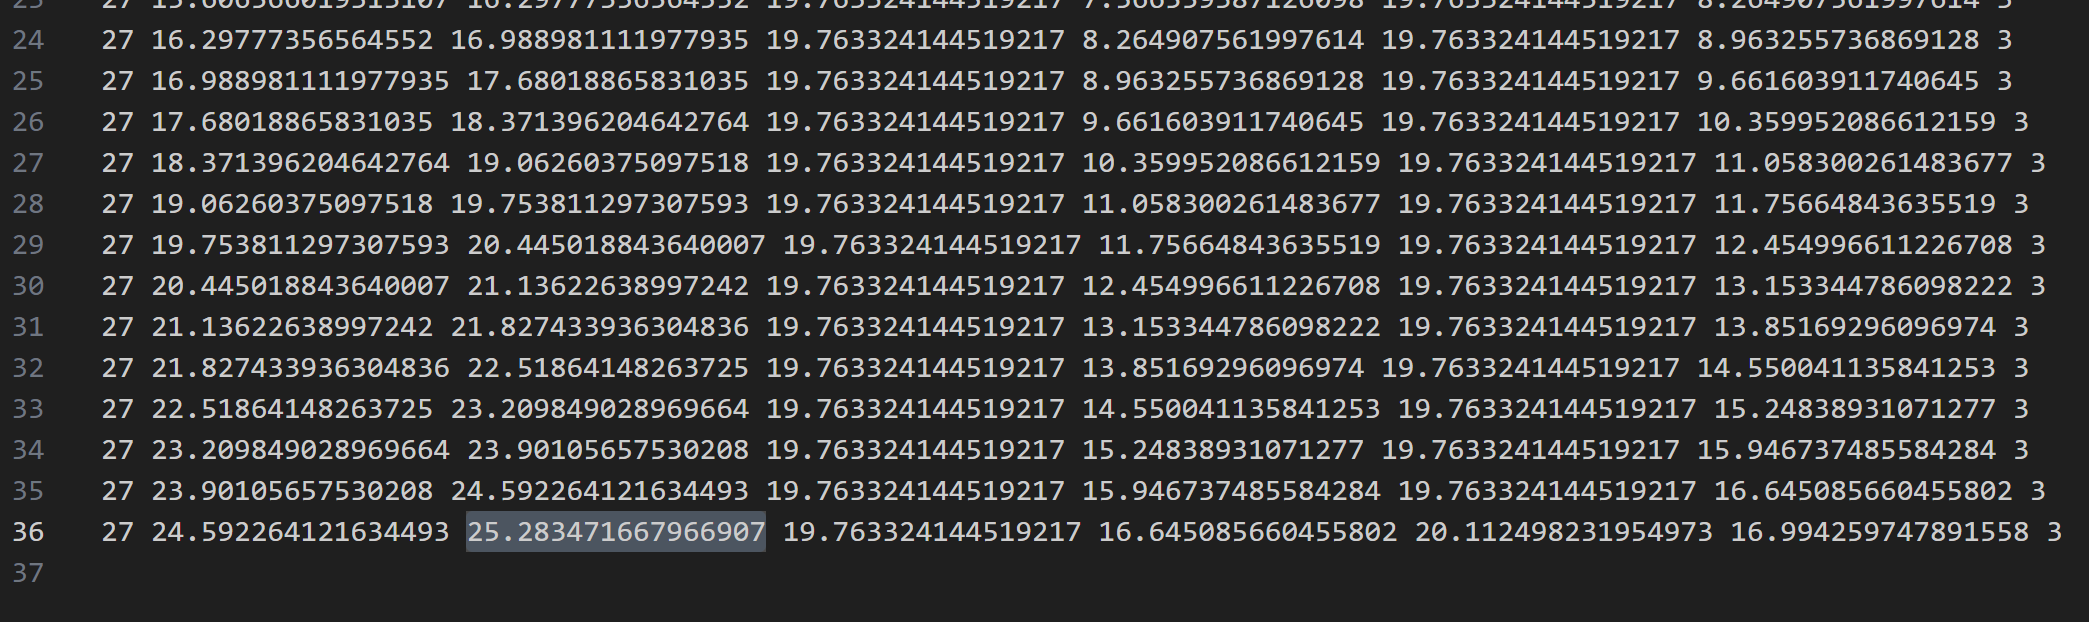
\includegraphics[scale=0.2]{report-template/images/source_fast.png}}

\caption{Pedestrian Travel Time}
\end{figure}

\end{task}